% ------------------------------------------------------------------------------
% Chapter 6 : Design and Implementation Storyboard
% ------------------------------------------------------------------------------
\setlength{\parindent}{4em}
\setlength{\parskip}{1em}

In this chapter, we are going to see scientific work carried out during this thesis. Implementation of this thesis is divided into two parts, training phase and prediction phase. In implementation, host and target platform is same that is Raspberry Pi 3B. It is referred as host platform in training framework and target platform in prediction framework. We will cover all technical details and methods used for each block in these frameworks.

\par First, we will look for the training phase. In training phase, an application is  feed to LLVM and then using LLVM and measurement tools, performance is measured at each phase on host platform. Same process is applied for wide number of application program written in programming language C/C++ to collect the training data. Following diagram \ref{fig:training} illustrate the training phase framework to collect the database. In further every component of framework is discussed in detail.

\begin{figure}[h!]
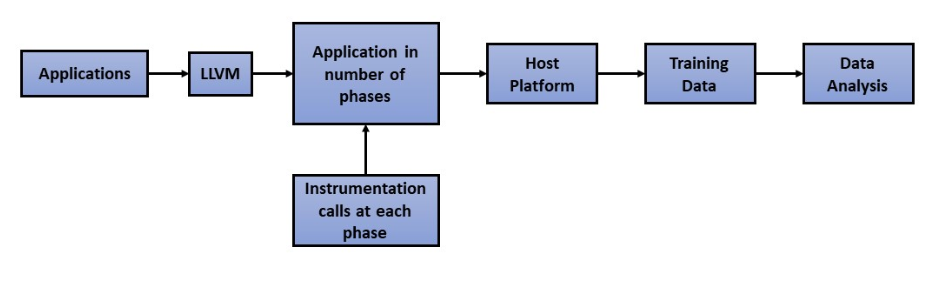
\includegraphics[width=14cm, height=5cm]{./images/training}
\centering
\caption{Training phase framework}
\label{fig:training}
\end{figure}

\section{Hardware platform}
In this thesis work, performance measurement for wide number of software applications are performed on Raspberry Pi 3B. Broadcom chip BCM2837 is used as SoC in Raspberry Pi 3B. This SoC uses ARM Cortex A53 quad core processor with 1 Giga Bytes of memory. It works on 1.2 GHz frequency. It supports MicroSD card for operating system and storing the data. Operating system used during this on Raspberry board was Raspbian Jessie which is open source license.

\par Processor on SoC of Raspberry is ARM Cortex A53. It is high efficiency processor for applications such automotive, mobile, DTV, networking, storage, aerospace and many more. It is based on Armv8-A architecture. It is quad core with Symmetrical Multiprocessing(SMP) within a single processor cluster, and multiple coherent SMP processor clusters through AMBA 4 technology[arm link a53]. Cortex A53 supports AARCH32 as well as AARCH64 instruction set architecture. It has full backward compatibility with Armv7 and it has 64 bit support. Raspbian Jessie is 32 bit OS and it was primary operating system during the thesis work. As it is 32 bit operating system, Cortex A53 was running on backward compatibility on Armv7 32 bit mode with AARCH32 ISA. It was not possible to use 64 bit mode with AARCH64 ISA. Following diagram \ref{fig:a53} from ARM[] illustrate the Cortex A53.

\begin{figure}[h!]
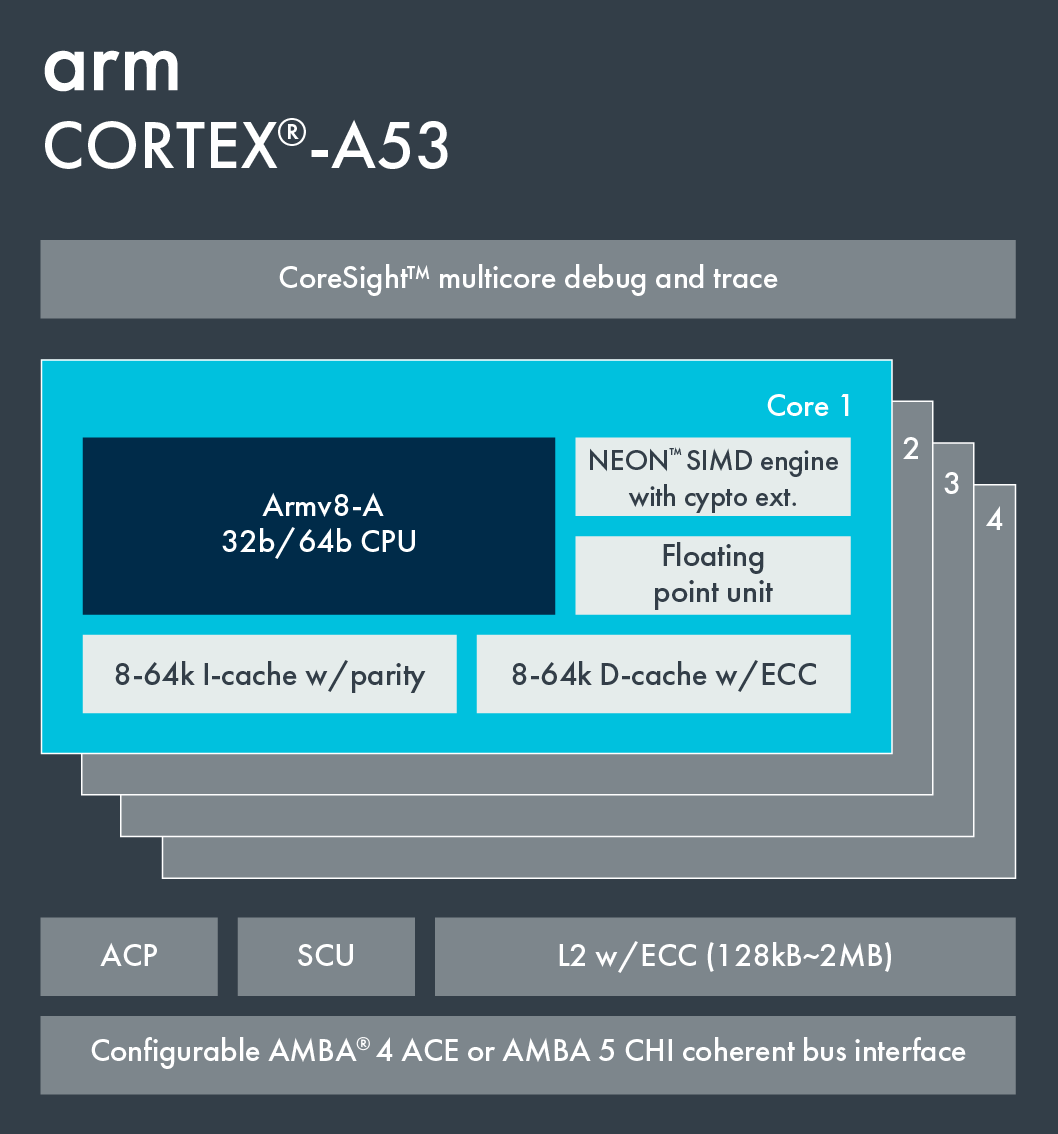
\includegraphics[width=8cm, height=12cm]{./images/A53}
\centering
\caption{Cortex A53[]}
\label{fig:a53}
\end{figure}

\par Cortex A53 has two level of cache hierarchy. Each core has level1 individual cache of 32kB. Level2 cache is unified for all cores with size of 512kB. As Raspberry was running on AARCH32 ISA, it was using AARCH32 PMU registers for hardware performance counters. Raspberry pi 3B has 14 hardware performance counter accesable through PMU. All hardware performance counters details we are going to see in upcoming chapter. 

\section{Training Set}
Validation of any learning based algorithm is depend upon the choice of training data. Insufficient of training data causes over interpretation and overfitting for learning model. For performance prediction, we need large number of diverse programs which contains the algorithms which are used in typical basic building block of software development of application.Good training data should have following properties, 

\begin{itemize}
\item[$\bullet$] Each workload included in training set should good representative of workload faced during prediction phase.
\item[$\bullet$] Variety of workload should be large enough to cover application interest.
\item[$\bullet$] Overall number of workload should be large enough to avoid overfitting problems in general.
\end{itemize}

\par In this thesis work, for performance prediction approach, We are using programs from ACM-ICPC[link] and SanFoundry[]. ACM-ICPC is the largest and prestigious progamming contest in which hundreds of programming problems are created and solutions are made public open source form. It provides great resource for program mining. Also some of the programs are taken from Sanfoundry. We are using total 264 programs from ACM-ICPC and Sanfoundry. Table shown below is breakdown of training set with respect to application domains.

\begin{tabular}{|l|c|r|p{1.7cm}|}
  \hline
  \textbf{Application Domains} & \textbf{Number of Programs}\\
  \hline
  Combinatorial problems & 27\\
  \hline
  Data structure & 34\\
  \hline
  Dynamic programming & 14\\
  \hline
  Geometry & 25\\
  \hline
  Graph & 30\\
  \hline
  Numerical problems & 30\\
  \hline
  String & 31\\
  \hline
  Miscellaneous & 48\\
  \hline
\end{tabular}

\par Programs in combinatorial problems involves finding a grouping, ordering or assignment algorithms. Data structure program contains particular way of storing and organizing information and retrieve it most productively. Dynamic programming problems are regarding solving complex problems into simpler subproblems.Solving each subproblem once and storing their solutions using memory based data structures. Geometric programs contains algorithms for solving geometric problems. There various programs in graph categories such as shortest path, graph search, network flow, etc. Programs such as calculus, linear algebra, floating point arithmatic operations, etc are involved in numerical problems. Problems in string category consist tasks such as parsing, encryption, decryption, etc. Finally, problems consist miscellaneous types complete the rest of training set. All these applications in training set are based C/C++ programming language. C/C++ programming languages is high level language. 

\section{Measurement Tool}

To measure the performance of the application on hardware platforms, performance measurement tools are used. These performance measurement tools extract the information from the PMU of the processor. PMU contains the hardware performance counters to monitor and count the microarchitecture events caused during the execution of software or application. There many measurement tools are available in market such PERF, PAPI, OProfile, gprof, ARM Streamline, etc. Some of them are open source licensed or paid licensed, the can be command line based, graphical user interface tools or APIs. We have seen basic information about performance measurements tools such as PERF, PAPI and ARM Streamline performance analyzer in chapter Basics. We will see basic use of each tool in following section. We are going to use following code block to see how to use these measurement tools in our environment. This example converts decimal number into binary number in recursive function. It is written in C programming language. It is compiled on GCC v4.9. 

\begin{lstlisting}
#include <stdio.h>
int convert(int);
int main()
{
long int i,bin;
for (i=0;i<50000;i++){
    bin = convert(i);
}
return 0;
}
// Function to convert number in binary.
int convert(int dec)
{
    if (dec == 0)
    {
        return 0;
    }
    else
    {
        return (dec % 2 + 10 * convert(dec / 2));
    }
}
\end{lstlisting}

\subsection{How to use PERF?}
In this thesis we used PERF v3.16 to measure the performance on Raspbian Operating system. Hardware platform has ARM Cortex A53 quad core processor in Raspberry pi 3B. We are going to use above program where its performance is going to be measure using PERF. 

  \textbf{Step 1: List of available hardware performance counters}
  
\begin{lstlisting}
 $ perf_3.16 list
 
List of pre-defined events (to be used in -e):
  cpu-cycles OR cycles                               [Hardware event]
  instructions                                       [Hardware event]
  cache-references                                   [Hardware event]
  cache-misses                                       [Hardware event]
  branch-instructions OR branches                    [Hardware event]
  branch-misses                                      [Hardware event]
  bus-cycles                                         [Hardware event]

  L1-dcache-loads                                    [Hardware cache event]
  L1-dcache-load-misses                              [Hardware cache event]
  L1-dcache-stores                                   [Hardware cache event]
  L1-dcache-store-misses                             [Hardware cache event]
  L1-icache-loads                                    [Hardware cache event]
  L1-icache-load-misses                              [Hardware cache event]
  LLC-loads                                          [Hardware cache event]
  LLC-load-misses                                    [Hardware cache event]
  LLC-stores                                         [Hardware cache event]
  LLC-store-misses                                   [Hardware cache event]
  dTLB-load-misses                                   [Hardware cache event]
  dTLB-store-misses                                  [Hardware cache event]
  iTLB-load-misses                                   [Hardware cache event]
  branch-loads                                       [Hardware cache event]
  branch-load-misses                                 [Hardware cache event]

\end{lstlisting}

This command shows the number of available hardware events, software events and kernel PMU events on command line terminal of Raspbian. You can see all hardware events listed by command. As Cortex A53 supports only 14 hardware performance counters. In above results some of the hardware counters are repeated with difference in name. For example, L1-dcache-load-misses and L1-dcache-store-misses, L1-dcache-stores  and L1-icache-loads, and branch-load-misses and branch-misses.

\textbf{Step 2: Measuring the performance of application}

\begin{lstlisting}
$ sudo perf_3.16 state -e cycles,instructions,cache-misses,
 branches,branch-misses -C 2 ./runme_large

Performance counter stats for 'CPU(s) 2':     
1,654,827,425      cycles                        
1,397,787,969      instructions              #    0.84  insns per cycle                    
3,528     	 cache-misses                                                       
94,047,959     	 branches                                                             
2,669,120    	 branch-misses          #    2.84% of all branches              
2.445278109 seconds time elapsed
\end{lstlisting}

\par Above C code is builded using GCC compiler and named executable as 'runme\_large'. Perf command options such as '-e' allow to insert events to be measured and '-C' option allows to collect the performance data for single CPU or for overall CPU in SoC. By using step 1, user can include events to be measured from list. In above step 2, We are measuring the performance of 'runme\_large' executable of decimal to binary program. With option 'e', we are measuring the total cycle, total instructions, cache-misses, branches and branches misses. Performance data for these events is collected from specified CPU i.e. 2 using '-C' option. 

\par PERF is also can be use to monitor live performance of software as well as operating systems. PERF provide many wide command line option with PERF commands to provide performance data to user. It is Linux tool which is available free of cost to use. Though only 14 hardware counters are available in Cortex A53 processor and only 6 counters can be accessed at time, PERF allows to use all hardware counter at same time with multiplexing but performance data may not accurate. 

\par In above example, only 5 hardware performance counters are monitored and data extracted from them for given specific application i.e. decimal to binary converter. To get values of other hardware performance counters, same command can be used as mentioned in Step 2 but with different or remaining hardware performance counters and execute new command to get more information of other hardware performance counters. 

\subsection{How to use PAPI}
PAPI is acronym for Performance Application Programming Interface. As its name suggests, it is combination of API and performance. PAPI provides APIs to measure performance of application or software. It provides interface for software designers and application engineers to hardware performance counter of processor. These APIs are need to be inserted in to code of application or software. PAPI provides  low level and high level APIs. Low level APIs manages events into user defined groups. These APIs provide fine grained measurements. Also these are well controlled APIs with increase in efficiency and functionality. 

\par In this thesis work we used PAPI v5.6.1.0 during the selection process of measurement tool. PAPI tool is available free on Linux environment, Raspbian. Following steps describes the use of PAPI calls in above sample code of decimal to binary conversion. 

  \textbf{Step 1: List of available hardware performance counters}
  
\begin{lstlisting}
$ papi_avail

Available PAPI preset and user defined events plus hardware information.
---------------------------------------------------------------------
PAPI version             : 5.6.1.0
Operating system         : Linux 4.9.78-v7+
Vendor string and code   : ARM (7, 0x7)
Model string and code    : ARMv7 Processor rev 4 (v7l) (4, 0x4)
CPU revision             : 4.000000
CPUID                    : Family/Model/Stepping 7/3331/0, 0x07/0xd03/0x00
CPU Max MHz              : 1200
CPU Min MHz              : 600
Total cores              : 4
SMT threads per core     : 1
Cores per socket         : 4
Sockets                  : 1
Cores per NUMA region    : 4
NUMA regions             : 0
Running in a VM          : no
Number Hardware Counters : 6
Max Multiplex Counters   : 384
Fast counter read (rdpmc): no
---------------------------------------------------------------------

=====================================================================
  PAPI Preset Events
=====================================================================
    Name        Code    Avail Deriv Description (Note)
PAPI_L1_DCM  0x80000000  Yes   Yes  Level 1 data cache misses
PAPI_L1_ICM  0x80000001  Yes   No   Level 1 instruction cache misses
PAPI_L2_DCM  0x80000002  Yes   No   Level 2 data cache misses
PAPI_TLB_DM  0x80000014  Yes   No   Data translation lookaside buffer misses
PAPI_TLB_IM  0x80000015  Yes   No   Instruction translation lookaside buffer misses
PAPI_HW_INT  0x80000029  Yes   No   Hardware interrupts
PAPI_BR_MSP  0x8000002e  Yes   No   Conditional branch instructions mispredicted
PAPI_TOT_INS 0x80000032  Yes   No   Instructions completed
PAPI_LD_INS  0x80000035  Yes   No   Load instructions
PAPI_SR_INS  0x80000036  Yes   No   Store instructions
PAPI_BR_INS  0x80000037  Yes   No   Branch instructions
PAPI_TOT_CYC 0x8000003b  Yes   No   Total cycles
PAPI_L1_DCA  0x80000040  Yes   No   Level 1 data cache accesses
PAPI_L2_DCA  0x80000041  Yes   No   Level 2 data cache accesses
---------------------------------------------------------------------
Of 108 possible events, 14 are available, of which 1 is derived.

\end{lstlisting}

\par Step 1 shows all hardware performance counters available in Cortex A53. It shows total 14 hardware performance counters are available to use in given processor. Unlike PERF, PAPI allows only 6 hardware performance counters to be accessed at time using APIs. It also shows the processor information. 

  \textbf{Step 2: Inserting API calls in code}
  
\begin{lstlisting}
#include "papi.h"
#include <stdio.h>
int convert(int);
int main()
{
/*Number of hardware counters*/
int num_hw_ctr=5;
/*List of hardware counters*/
int Events[5]={PAPI_TOT_CYC,PAPI_TOT_INS,PAPI_L2_DCM,PAPI_BR_INS,PAPI_BR_MSP};
long_long values[5];

if(PAPI_start_counters(Events,num_hw_ctr)!=PAPI_OK)
        printf("Error in starting counter");
long int i,bin;
for (i=0;i<50000;i++){

    bin = convert(i);

}
if(PAPI_stop_counters(values,num_hw_ctr)!=PAPI_OK)
        printf("Error in stopping counter");
printf("cycles: %lld\n,instructions: %lld\n, L2 cache miss: %lld\n, branches: %lld\n, branch misses: %lld\n",values[0],values[1],values[2],values[3],values[4]);
return 0;
}

int convert(int dec)
{
    if (dec == 0)
    {
        return 0;
    }
    else
    {
        return (dec % 2 + 10 * convert(dec / 2));
    }
}

\end{lstlisting}

\par As we can see in above code PAPI APIs are used in code with PAPI library i.e. PAPI header file for API calls. As we can see total number of hardware counters are already mentioned in code with their names and accessed using API calls to hardware performance counters of PMU of the processor. In above code with PAPI API calls we are measuring the total number of cycles, total number of instructions, Level 2 data cache miss, total number of branches and total number of branches mispredicted for decimal to binary code. 

  \textbf{Step 3: Execute the code}

\begin{lstlisting}
 $sudo taskset -c 2 ./runme_large
 
 cycles:		1653593201,
 instructions:	1397640501,
 L2 cache miss:	2178,
 branches:	137950307,
 branch misses:	2668136
\end{lstlisting}

\par PAPI API calls inserted in decimal to binary conversion code is compiled with GCC v4.9 on Raspbian and named to runme\_large executable. Executable need to be execute with super user. Above you can see the results in terms of hardware performance counters for decimal to binary converter code. All this data is collected on core 2 of Cortex A53's quad core processor using Linux command. 

\subsection{How to use Streamline}
Streamline Performance Analyzer tool is provided by ARM Inc. ARM designs most of the embedded processors and this tool helps to monitor the performance of the software or application on ARM processor. One the main reason to explore this tools is that the Raspberry Pi 3B contains the ARM Cortex A53 processor.  Streamline provides the system-wide visualizer, live capturing of the data with background processes and kernel process, it also shows the core wise heatmap to understand the application execution on core level. It also provides the information about call paths, functions, code after capture process. 

\par Streamline tool can not be used on Raspbian directly because it has higher system requirements which Raspberry does not supports. So it is installed on higher configures host PC. It communicate with the Raspberry, hardware platform using communication daemons installed on hardware platform. Barman and Gator these to daemons can be used to communicate. Barman is use to monitor the performance of bare metal system where as Gator is used for board with operating systems on it. In our case, we are using Raspbian operating system so we are using Gator daemon while exploring the performance tools for this thesis work. Using Gator daemon, Streamline collect the performance data for hardware platform on Host PC. Usage steps of Streamline is as following,

  \textbf{Step 1: Start Gator on hardware platform}
\begin{lstlisting}
$ sudo insmod /home/pi/gator/driver/gator.ko
$ sudo /home/pi/gator/daemon/gatord &
\end{lstlisting}

To start the communication between Host PC and hardware platform, Gator driver and daemon should be running on hardware platform. Hardware platform can be configured by adding credentials for Raspbian such as IP address of hardware platform, username and password. Daemon collects the performance related information from hardware performance counters. Once communication is established the hardware performance counters can be selected in Stream line on Host PC. 

To select the hardware performance counters, counter configuration button can be used on Streamline. In new window it shows the available hardware counters and 6 hardware counters can be selected.

To capture the performance on hardware platform, capture button is pressed and data capturing starts but mean while it make sure that the application whos performance need to be measure  should also execute during this time of capturing the data. 

After capturing the data, capture can be stopped and performance data can analyzed using window selector. 

\subsection{Comparison of Measurement Tools}

In this subsection, we are going to see the comparison between explored performance measurement tools. Comparison is based on parameters like live analysis feature, event based sampling, use of annotations, API calls in code, measurement time, cost and availability. 


\begin{tabular}{|l|c|r|p{1.7cm}|}
  \hline
  \textbf{Parameters} & \textbf{PERF} & \textbf{PAPI} & \textbf{Streamline}\\
  \hline
  \textbf{Live analysis} & Possible & Not Possible & Possible\\
  \hline
  \textbf{Event based sampling} & Possible & Not possible & Possible\\
  \hline
  \textbf{Annotations} & Possible & Not possible & Possible\\
  \hline
  \textbf{API calls} & Not possible & Possible & Not possible\\
  \hline
  \textbf{Measurment time} & Relatively fast & Relatively fast & Relatively slow\\
  \hline
  \textbf{Cost and Availability} & Free & Free & Paid\\
  \hline
\end{tabular}

\par We also measured the hardware performance counter values on PERF, PAPI and Streamline for applications like BasicMath, BitCount and Qsort for short range of inputs. Following results in figures \ref{fig:tool_results} shows the few hardware counters values extracted from these tools and their comparisons with respect to accuracy to each others. 


\begin{figure}[h!]
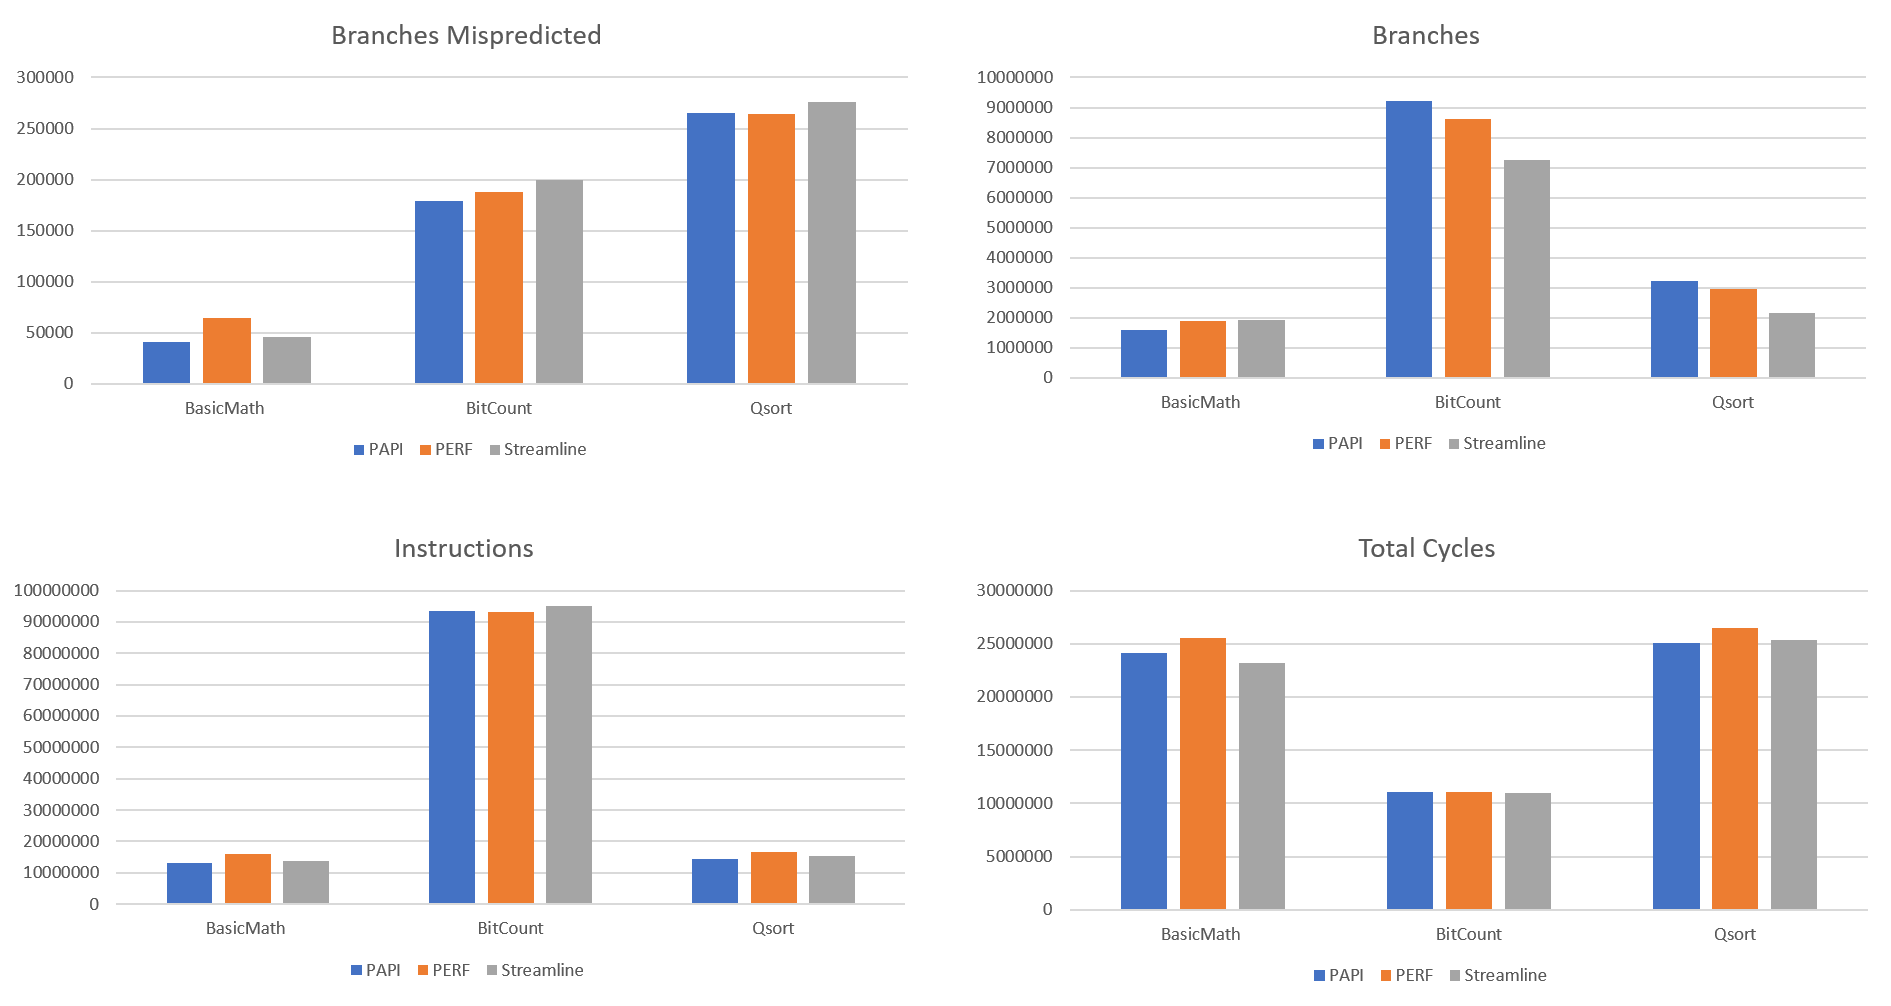
\includegraphics[width=14cm, height=14cm]{./images/tool_result}
\centering
\caption{Comparison of hardware performance counter values on PERF, PAPI and Steamline for BasicMath, BitCount and Qsort applications}
\label{fig:tool_results}
\end{figure}

\subsection{Tool selection}

We explored three performance measurement tools. We compared them with respect to parameters such as live analysis, annotations, API calls, Cost and etc. Also we compared the values captures by these tools on three different application with few hardware performance counters. All three tools have their own distinguish features such GUI for Streamline, Multiple counters at a time in PERF and API calls in PAPI. 

\par But most important hing is which is suitable for learning model. Because main objective of this thesis is to predict the performance. Which tools can be best fitted in this objective where performance data need to be collected at phase level of applications or software with LLVM tool chains. For that tool need to be have fast response time, easy to use and available free also. And most important, it should measure data at phase level. By considering all these factors, Streamline is slow in response and to collect large training data it will consume time and also it is paid. So Streamline can not be used here. Whereas PERF is open source tool, fast response but main disadvantage of PERF is that it is not able to measure performance data at phase level of software. And hence PAPI is best suitable tool to collect that performance data that can be used as training data. PAPI provides API calls that be inserted in phases of application using LLVM toolchain. Also response time is fast ans it is available free of cost.

\section{Grouping of the Counters}
In this thesis with respect to state of the art, we are going to see grouping of the hardware performance counters. Grouping of hardware performance counter is essential because in this thesis, we going to collect the training data in thirteen dimensional as input parameters and 1 dimensional output to understand the relationship between them. But measure concern is that total number of hardware performance counters available in PMU of Cortex A53 are 14. And we selected the tool for performance measurement is PAPI. PAPI allowed only 6 hardware performance counters to access at a time. So wee need to group hardware counters. 

\subsubsection{Multiple Measurements}
To test the PAPI as performance measurement tool, in this thesis work as small experiment, we used PAPI API calls in benchmark programs. In this experiment, we used PAPI high level calls in benchmark programs from MiBench[] and execute the same programs for 100 times to observe the consistency of values counted by PAPI tool for every execution. This data is gathered for complete program, not for different phases of programs. The following figure \ref{fig:grp_4} is resulted from execution of Basicmath program from MiBench benchmark suite. Program is executed 100 times and every time the total cycles, total instructions, level 2 cache miss, level 2 cache access, level 1 data cache miss and level 1 instruction cache miss, these hardware counters are measured for resulted figure. We also collected the data for other hardware counters for every execution and observed the consistency of PAPI tool in terms of performance measurement. 

\begin{figure}[h!]
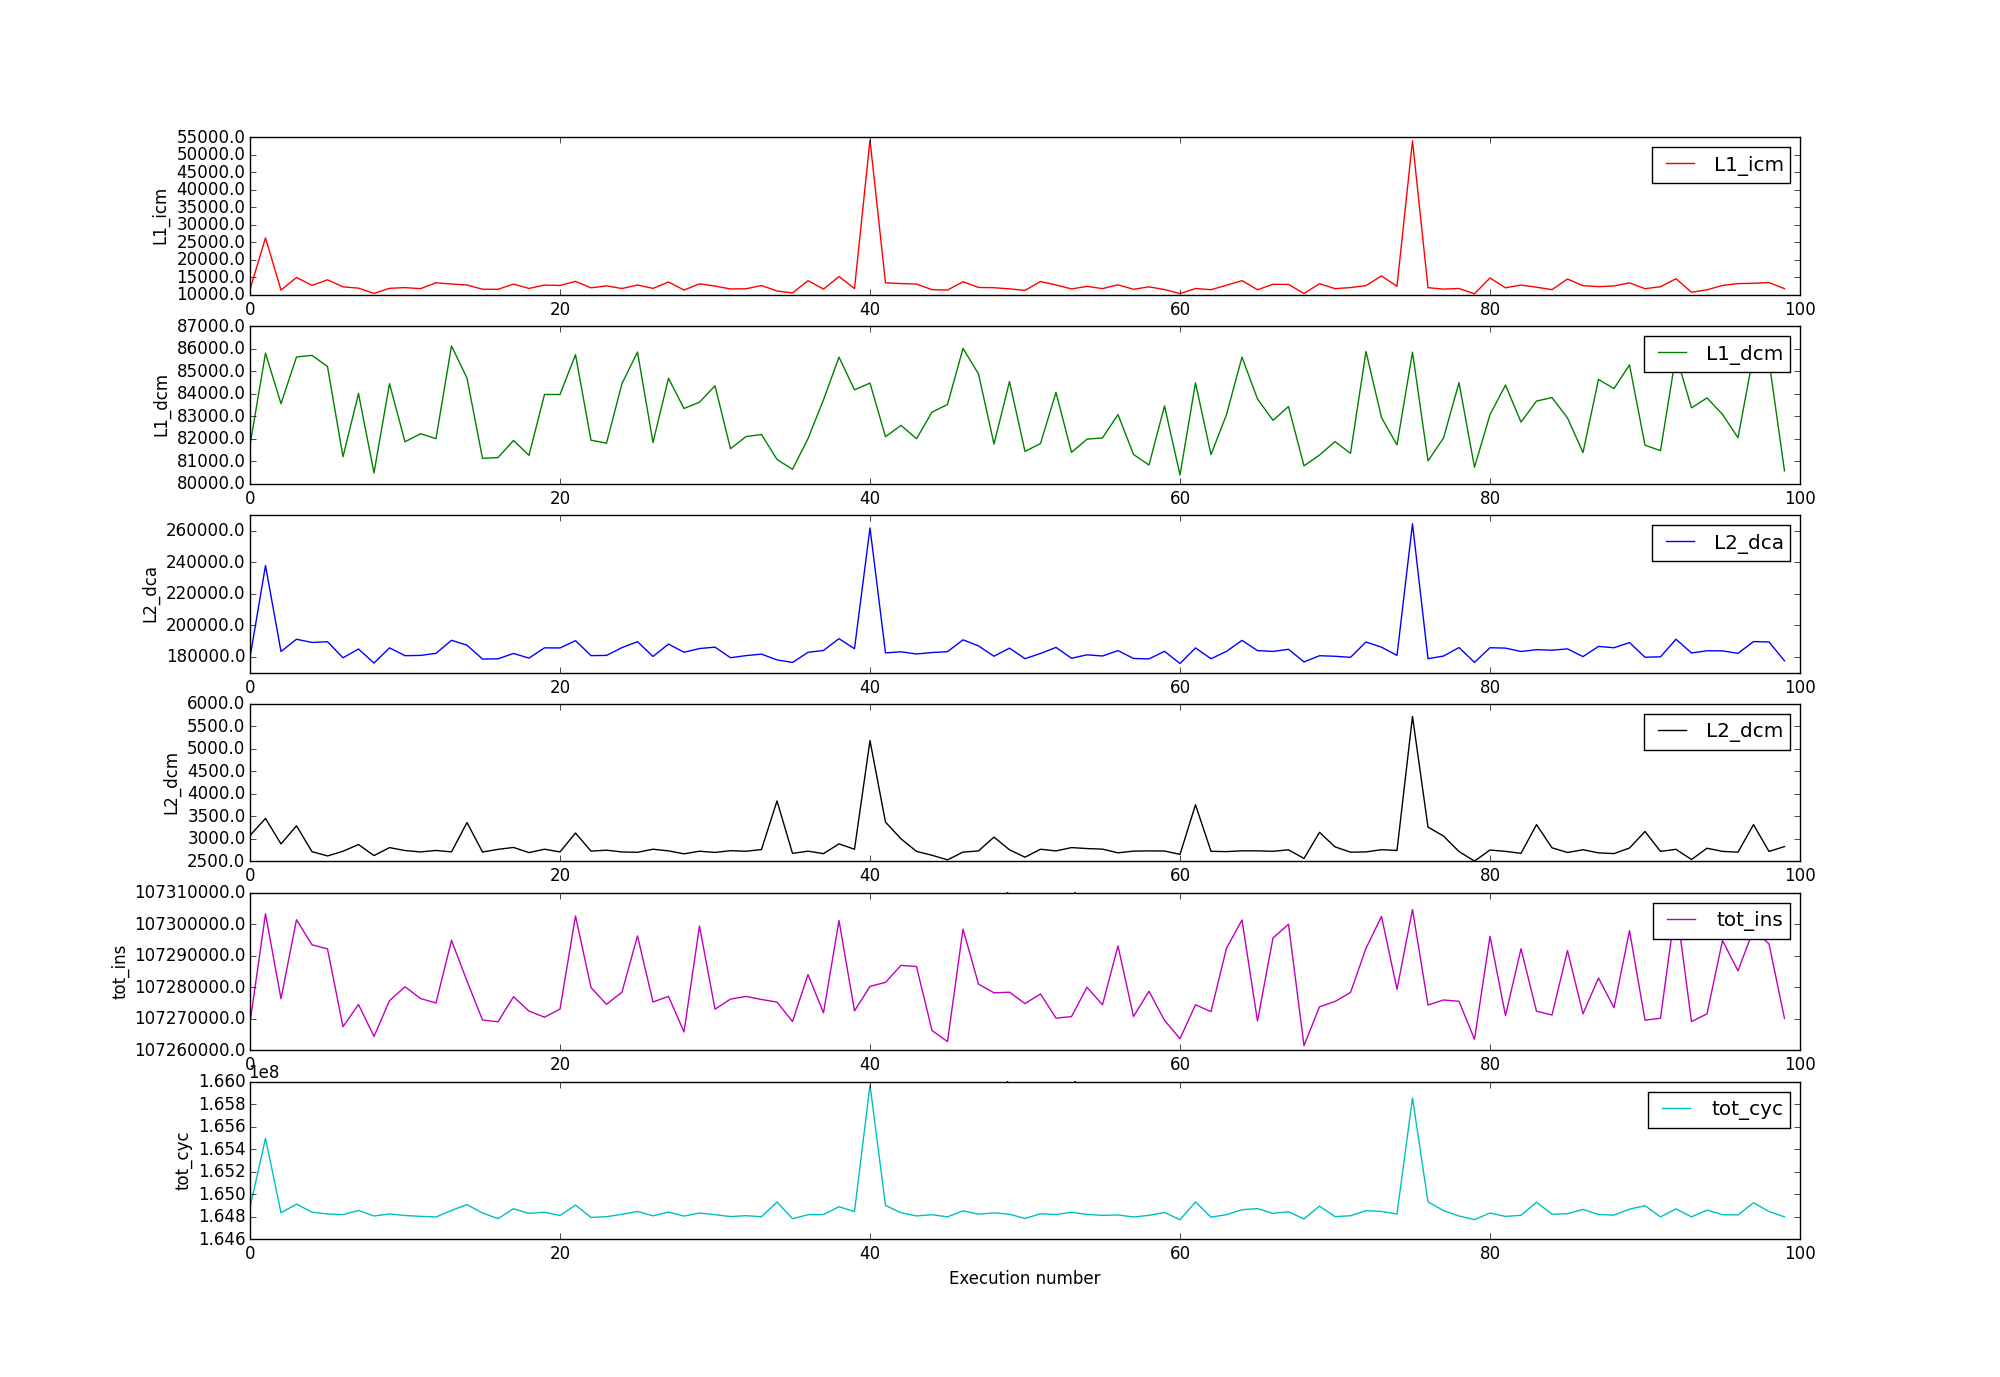
\includegraphics[width=14cm, height=14cm]{./images/grp_4}
\centering
\caption{100 time execution of same program using PAPI}
\label{fig:grp_4}
\end{figure}

\ we also calculated and plotted the percentage in hardware counter values with respect to average value. Following figure \ref{fig:grp_4_perc_change} shows the change in percentage for hardware counter discussed in above paragraph. As we can see the figure \ref{fig:grp_4_perc_change}, percentage change in hardware performance counter measurement is vary with respect microarchitectural events, but change is acceptable because there are might be some kernel process is active in background. While measurement we made sure to avoid external interruption during the measurement and measurements are taken on isolated core of Cortex A53.  

\begin{figure}[h!]
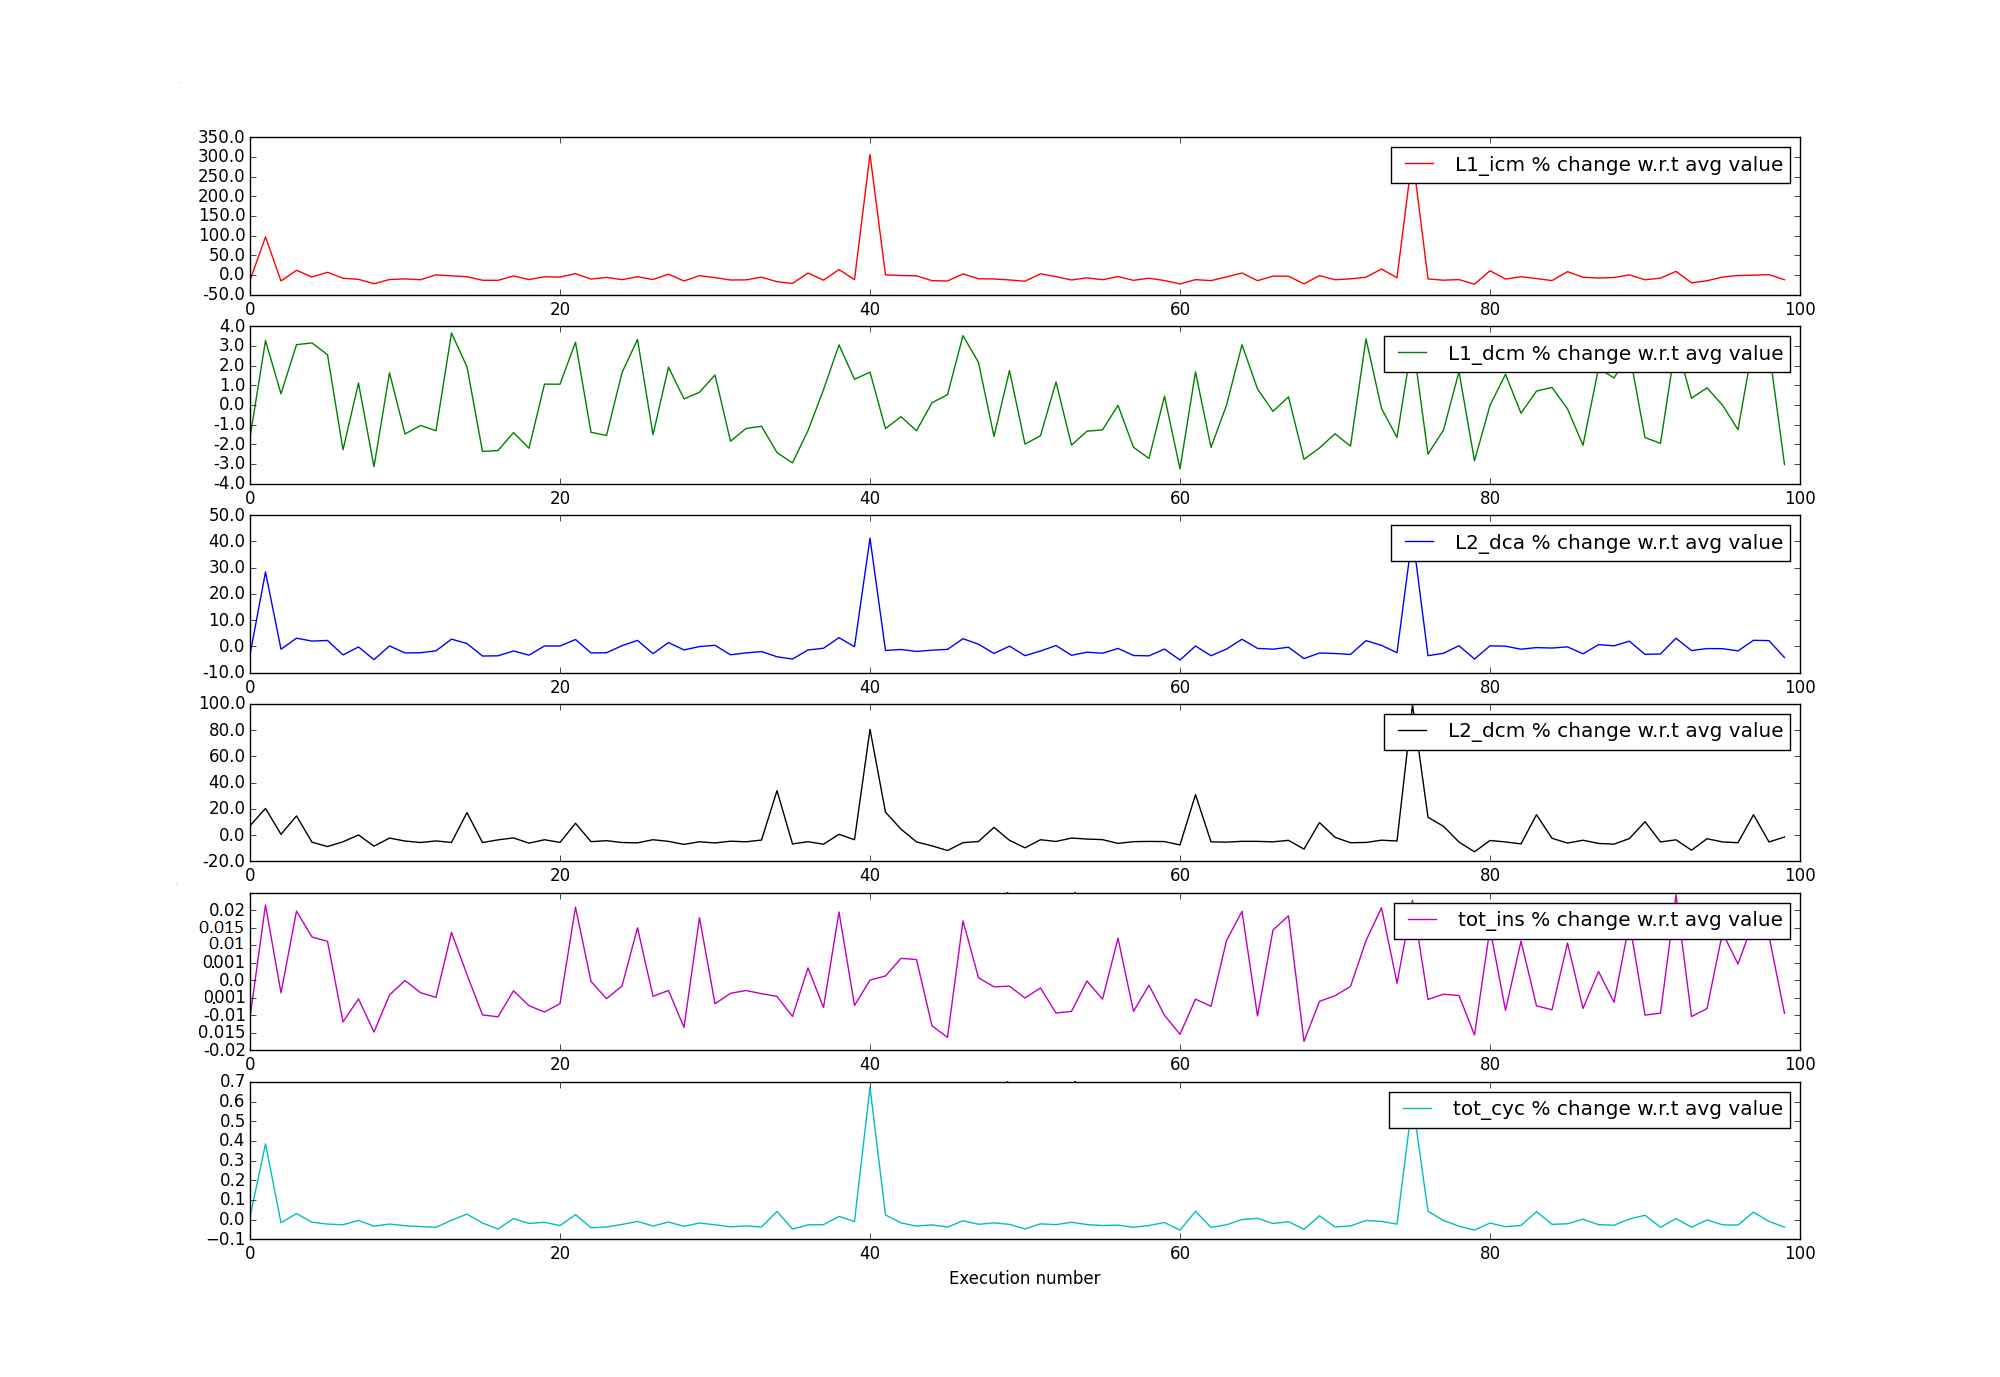
\includegraphics[width=14cm, height=14cm]{./images/grp_4_perc_change}
\centering
\caption{100 time execution of same program using PAPI}
\label{fig:grp_4_perc_change}
\end{figure}

\subsubsection{Counter grouping}
In order to observe the behavior of hardware counters on total cycles, we performed grouping of the hardware counters and number of hardware counters in each group are equal to 6 or less than 6 due restriction of accessing counters at a same time. In following table, you can see different combinations. These combinations are made in order to understand the impact of them on total number of cycles for same programs but with different groups.  We performed small experiment on Raspberry to conclude the final groups for hardware counter which are going to use in further processing like collecting training data and creating the framework. 

\begin{tabular}{|l|c|r|p{1.7cm}|}
  \hline
  \textbf{Sr. No.} & \textbf{Combinations}\\
  \hline
  1 & Branch instructions, Branch mispredicted, Total instructions, Hardware interrupts, L1 instruction cache miss, Total Cycles\\
  \hline
  2 & L2 data cache accesses, L2 data cache miss, Load instructions, Store instructions, Total cycles, Branch mispredicted\\
  \hline
  3 & TLB data miss, TLB instruction miss,  Branch mispredicted, L2 data cache miss, total cycles, Total instructions \\
  \hline
  4 & L1 instruction cache miss, L1 data cache miss, L2 data cache access, L2 data cache miss, total instructions, total cycles\\
  \hline
 5 & L1 instruction cache miss, L1 data cache miss, L2 data cache access, L2 data cache miss, Hardware interrupts, Total cycles\\
  \hline
  6 & L1 instruction cache miss, L1 data cache miss, L2 data cache access, L2 data cache miss, L1 data cache access, Total cycles \\
  \hline
  7 & Branch instructions, Branch mispredicted, Load instructions, Store instructions, Total cycles\\
  \hline
  8 & Hardware interrupts, TLB data miss, TLB instruction miss, Total cycles \\
  \hline
\end{tabular}


\par After running these combination of counters mentioned in above table are run on Raspberry for multiple time for multiple programs. While collecting the results, we monitored the impact of hardware counters on total number of cycles. From above combinations, we selected the combination 6,7 and 8. In combination of 6, we can see all hardware counters are related to caches. If level 1 cache is missed then it can be hit for level 2 or can be miss. By combining all cache related hardware counters, their impact can be understandable on cycles. Combination 7 consists, hardware counters related to instructions such as store instructions, load instructions, total instruction as well as total branches and branch mispredicted, their impact can be observed on cycles. Same time remained counters are grouped together for example, TLB instruction and data miss and hardware interrupts. These group does not have much impact oh cycles. 

\section{Application in Phase levels}
Collect the performance data at phase level is one the primary challenge in this thesis work. It is backbone of this thesis work. Performance data is collected at phase level of application on hardware platform. Which helps to understand the software behavior and the performance at different phases on hardware platform. In this thesis work, this main objective is accomplished with LLVM tool chain and PAPI library. This framework collect fine-grain level of data from application executing on hardware platform. Also with this framework, user can change the granularity of phases, which helps to understand the behavior at different granularity level. In this thesis work, we are using LLVM v3.5. 

\par LLVM is collection of reusable compiler and toolchain technology. It provides the toolchains like compiler, assembler, linker, optimizer, and etc. We are going to use Clang, native compiler from LLVM. It supports C/C++/Objective-C programming languages. It compiles faster than GCC compiler and provides useful warning and error messages. It also provide static analyzing of code to find bugs. We are also going to use LLVM linker, LLD, whichis helpful to link all bitcode files generated by Clang compiler. LLVM optimizer, opt, it takes input files and run specified optimizations and analysis on it. We are also going to use llc, that is LLVM's static compiler. Which compiles the source inputs into assembly language of specified architecture. 

\subsection{Creating phases}
Collect the data at phase level of application, PAPI libraries are used. These PAPI libraries are embedded into LLVM toolchain and shared objective library is created to divide application in different phases as well as in basic blocks. 


\subsubsection{Finding the basic blocks}
LLVM allows to create LLVM pass framework. Most of the compiler's parts are exists in LLVM passes. LLVM passes perform the transformation and optimizations that make up the compiler. LLVM passes are subclasses of LLVM pass, there are many subclases such as ModulePass, FunctionPass, BasicBlockPass and many more passes, which gives the more information to system about what pass does and how it can be combined with other passes. Before that lets go through the more information about basic blocks. Basic blocks is traight lines of code sequence which consists one entry point and one exit point and in between this there are statement/s.

Using LLVM passes and PAPI API calls, PAPIInstrument shared library is created. This is created with LLVM passes like FunctionPass, BasicBlockPass, ModulePass, and InstructionPASS. Most basic and solid part is to find the number of basic block. This library provide option 'bbtrace' which shows the number of basic block. We can show in following command and result. We used same code as we mentioned in above section i.e. decimal to binary code. To get the list of basic blocks, code is compiled with Clang compiler and bitcode file generated for the code.

\begin{lstlisting}
$ opt -load $(INS_LIB) -bbtrace -analyze < dec_to_bin.bc > bbstats.log
$ cat bbstats.log

Printing analysis 'Basic Block Trace':
0: alloca 3 br 1 call 2 store 2 
1: br 1 icmp 1 load 1 
2: add 1 br 1 load 1 store 1 
3: add 1 br 1 load 1 store 1 
4: ret 1 
\end{lstlisting}

Using LLVM optimizer bitcode is analyzed and optimized. INS\_LIB is path to the shared library PAPIInstrument. Which provide option '\-bbtrace' to get the basic block. LLVM count and displays all basic blocks based on IR representeation code. Above results are generated for IR code decimal to binary conversion. Bitcode file consists the IR code representation of the code. Using this IR code representation basic blocks are counted.

\subsubsection{Adding instrumentation calls}
Now, we know how to find basic blocks from applications. Now main task is to insert performance measurement API calls of PAPI in these blocks. To measure the performance of each basic block is not feasible. It can cause more overhead because PAPI API calls also going to be part of it while executing the application on hardware platform. So we decided to combine number basic block and we called it as phase. Phase consist number of basic blocks which user can defined. In diagram \ref{fig:phase} illustrate the phases. In this figure \ref{fig:phase}, one phase consist 1000 basic blocks. And we called it granularity of 1000. Granularity can be increased or decreased. Last phase may contains 1000 basic blocks or less than basic block because last phase consist only remaining basic blocks in it. 

\begin{figure}[h!]
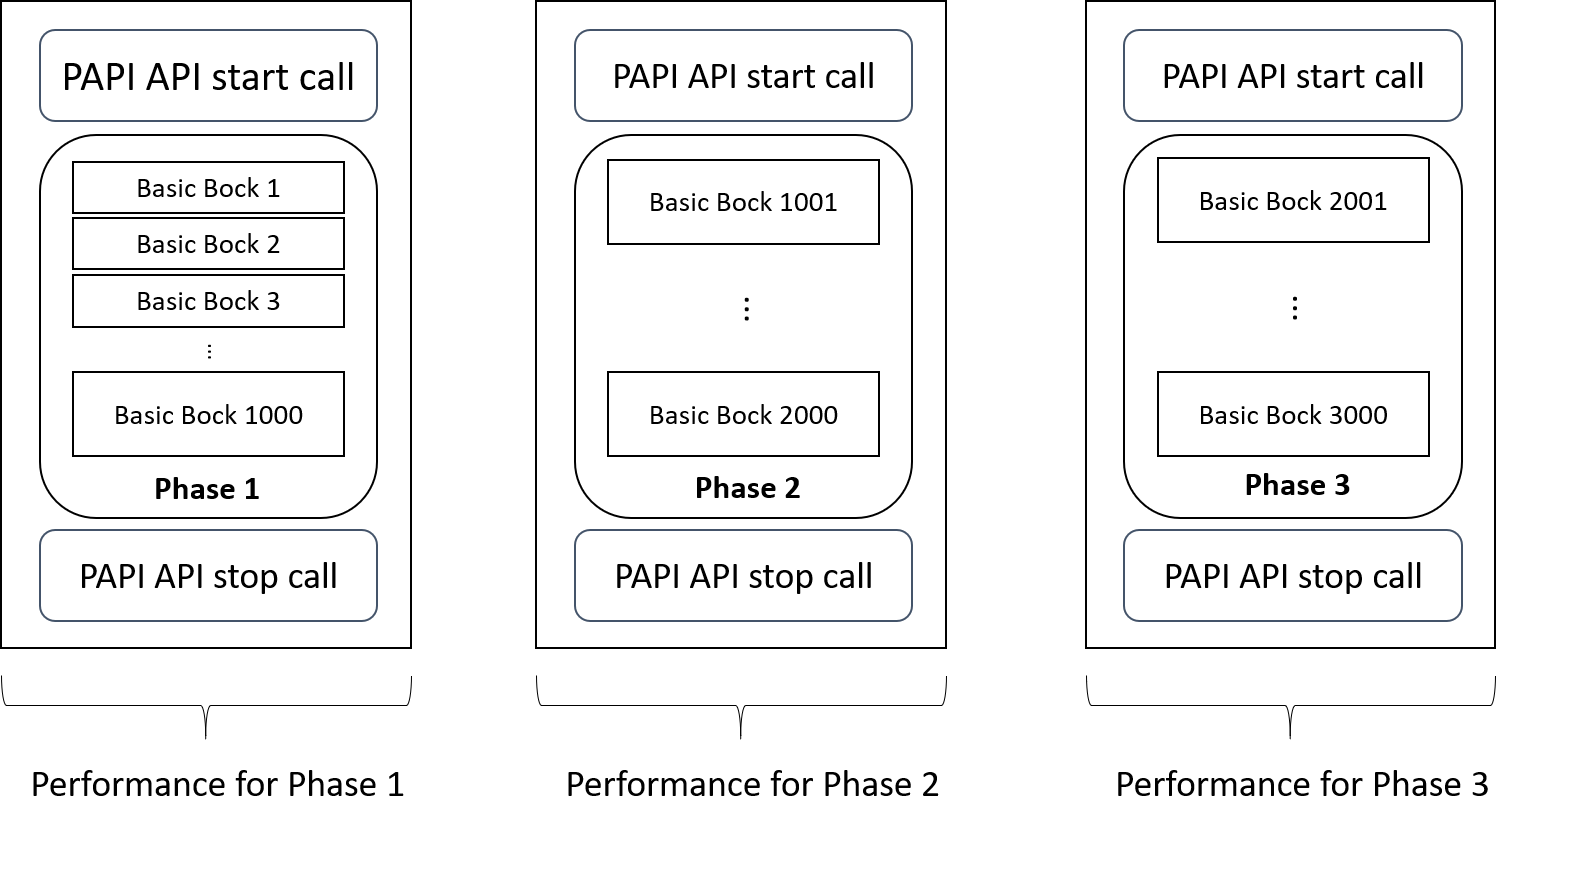
\includegraphics[width=13cm, height=10cm]{./images/phase}
\centering
\caption{Phases with granularity of 1000}
\label{fig:phase}
\end{figure}

\par Granularity of different sizes is possible due to PAPIInstrument library. Library combines the number of basic blocks based on defined granularity. For this it need additional source file of PAPI API calls to be linked with. First compiled code converted into bitcode and optimized using LLVM optimizer. PAPIInstrument library provide option 'papi\_instru\_bb'. This option need to be use while collecting performance at phase level. Following flow chart \ref{fig:flow} illustrate the creating phases and inserting performance call at start and i end of the phase. 

\begin{figure}[h!]
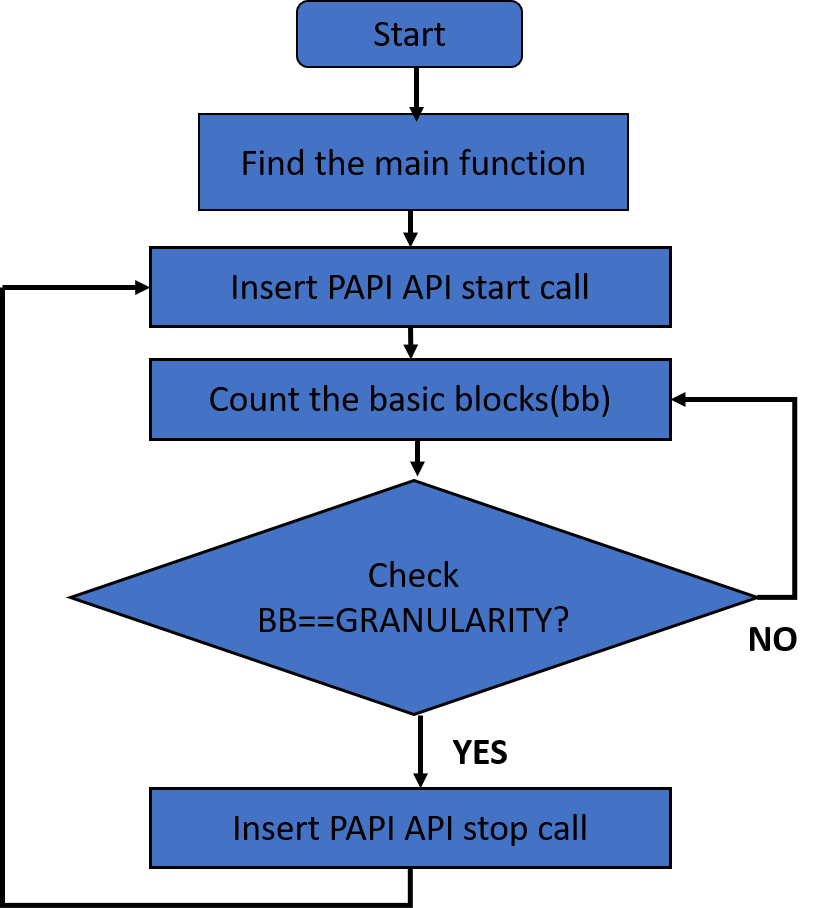
\includegraphics[width=10cm, height=13cm]{./images/flow}
\centering
\caption{Creating phases and adding performance calls}
\label{fig:flow}
\end{figure}

Followings are the instrumentation steps. All these steps are combined and composite into Makefile. This Makefile structure helps to create executable with single Linux command. INS\_LIB is the environmental variable which has the path of PAPIInstrument library set. 

  \textbf{Step 1: Compile the source files}
  \begin{lstlisting}
   $ clang -emit-llvm -g -I -c "source_file_name/s"
  \end{lstlisting}

In this step, LLVM compiler Clang compiles the source files which are written in C/C++ programming languages. Option \-emit\-llvm creates the bitcode file with .bc extension for each source file. 

  \textbf{Step 2: Link all bitcode files}
  \begin{lstlisting}
  $ llvm-link "source_files.bc" -o $(TARGET).linked.src.bc
  \end{lstlisting}

Step 2, uses llvm-link command from linker to link all bitcode files into single TARGET bitcode file. TARGET is name for executable gong to be created. Which will be single file resulted by linking all other bitcode files and that single file has local naming convention in this thesis work i.e. TARGET.linked.src.bc.

  \textbf{Step 3: }
  \begin{lstlisting}
  $ opt -load $(INS_LIB) -bbtrace -analyze < $(TARGET).linked.src.bc > bbstats.log
  \end{lstlisting}
  
  Step 3, Using optimzer and PAPIInstrument shared library, log file is created which has list of basic blocks. This step is optional. It only create log file of basic blocks. Instrumentation calls are not inserted during this step.
  
    \textbf{Step 4: }
  \begin{lstlisting}
  $ opt -load $(INS_LIB) -papi_instru_bb < $(TARGET).bc > $(TARGET).instru.bc
  \end{lstlisting}
  
  Step 4 adds instrumentation call at each phase level using PAPIInstrument library and create new bitcode file with .insru.bc extension with Target executable.

    \textbf{Step 5: }
  \begin{lstlisting}
   $ clang++ -emit-llvm -g -I $(PAPI_INC) -c papi_helper.cpp -o papi_helper.bc
  \end{lstlisting}
  
  In Step 5, bitcode for papi\_helper is created using Clang compiler. This papi\_helper consist the PAPI high level API calls. These API calls are going to inserted at each phase of the software or application of whos performance is going to collected.
  
 \textbf{Step 6: }
  \begin{lstlisting}
      $ llvm-link $(TARGET).instru.bc papi_helper.bc -o $(TARGET).linked.bc
  \end{lstlisting} 
  
  All bitcode files are linked using llvm linker like Target bitcode files with instrumentation call of bitcode of papi\_helper.  And single linked file is created with extension .linked.bc.
  
 \textbf{Step 7: }
  \begin{lstlisting}
$ llc -filetype=obj $(TARGET).linked.bc -o $(TARGET).o
  \end{lstlisting} 
  
  In Step 7, using LLVM static Compiler, LLC, which takes linked bitcode file as input and it compiled again with respect to target hardware architecture. It can be called object file and .o extension is given to compiled file with target executable name.
  
   \textbf{Step 8: }
  \begin{lstlisting}
 $ gcc $(TARGET).o -o $(TARGET) -L $PAPI_LIB -lpapi -lm
  \end{lstlisting} 
  
  Step 8 is the last step where executable for target is created. Where PAPI\_LIB is environmenatal variable consist path for PAPI libraries. 
  
\subsubsection{Automation to create Makefile}
All above steps are written in single makefile to create executable for single application. We have total 263 number of application from different domains and with single or multiple source files. To create makefile for each application can consume more time. So automation need to be created to make all makefiles. To execute each applications in this thesis work, it need at least 4 files. Source file, it can be either in C or C++, input file, in which consist all inputs for application which can be optional depends upon applications, Makefile and run executable to which contains the application executable. Also with each application we need papi\_helper file. We will see in coming section how to add the it using framework. 

\par We created two automation scripts using python and Linux Bash scripts. One automation screept is for single source file and another for multiple source files. Apart from that both have similar functionality. Both automation scripts removes the white spaces from source file names and create new name without white spaces. Renamed source file name is used as Target in makefile. These autotmation scripts make makefile for application with Target name as we discussed. These also create run executable file for Linux bash scripts which contains the target executable in it. These automation scripts are handy and less time consuming. 
  
\par Till now, we have seen PAPI tool and LLVM combination. And new PAPIInstrument library which creates the phases into application and insert performance measurement calls at start and end of phase. This is the backbone for upcoming frameworks, training and prediction framework.
  
\section{Framework to collect training data}
In this section, we are going to see framework which collects the training data with granularity. Prerequisite for this framework was grouping of hardware performance counters and instrumentation calls at phase level of applications. All these prerequisites are completed in previous session. One more thing, we need to understand is how granularity can effectively change with each group. 

\par As we discussed above, to insert instrumentation call at each phase, LLVM need papi\_helper file, which written in C++ programming language and it contains the granularity level as well as group of hardware counters. We have three groups of hardware counters and execution of same program need to be done three times with same granularity. For that we inserted automation script which is created using python. This scripts takes the hardware counter group and granularity as input. For example you can see it in following bash script. 

\begin{lstlisting}
#!/bin/bash

PAPI_EVENTS_BATCH_1=(PAPI_L1_DCM PAPI_L1_ICM PAPI_L2_DCM PAPI_L1_DCA PAPI_L2_DCA )
PAPI_EVENTS_BATCH_2=(PAPI_BR_MSP PAPI_BR_INS PAPI_TOT_INS PAPI_LD_INS PAPI_SR_INS)
PAPI_EVENTS_BATCH_3=(PAPI_TLB_DM PAPI_TLB_IM PAPI_HW_INT)

python $PY_UTIL/papi_helper_setup.py  ${PAPI_EVENTS_BATCH_1[@]} --granu 1000
python $PY_UTIL/papi_helper_setup.py  ${PAPI_EVENTS_BATCH_2[@]} --granu 1000
python $PY_UTIL/papi_helper_setup.py  ${PAPI_EVENTS_BATCH_3[@]} --granu 1000

\end{lstlisting}

This bash scripts uses python script i.e. papi\_helper\_setup.py to create papi\_helper file, which is going to use for instrumentation of applications. Path of the automation script is stored in environmental variable PY\_UTIL. This script uses template script to create papi\_helper with given hardware counters and granularity. Script require to input parameters. One is list of hardware performance counters and granularity in integer number. 

\par Now we will see the use of the training data framework. All application with makefile and run executables are store in training\_programs repository. Framework to collect training data has the path for training application repository stored. Another important change need to be made in framework is that whether user want to collect the training data on single core or on dual core with no load or full load. Following command can be use for single core and dual core modes. In dual core scenario, data is collected in two different environment. 
\begin{itemize}
\item[$\bullet$] No load
\item[$\bullet$] Full load
\end{itemize}

This command is for single core mode. Where core 2 is isolated and using this command user can force applications to execute on core 2.
\begin{lstlisting}
$ sudo taskset -c 2 ./run
\end{lstlisting}

Following command can use to collect the data on dual core. 
\begin{lstlisting}
$ sudo chrt -r 1 taskset -c 2,3 ./run
\end{lstlisting}

\textbf{No load}
\par In no load scenario, no background additional process is running. Only operating system is running on it i.e. Raspbian. Other two core, core 0 and core 1 are isolated from execution. Only core 2 and core 3 are active. All performance data is collected on these two cores. using framework. 

\textbf{Full load}
\par In full load scenario, same prerequisites are applied. Core 0 and core 1, are isolated and all operations are performed on core 2 and core 3. To make it full load scenario, background application is running on core 3. We use stream application[] to utilize the core 3. Application try to utilize core 3 completely in background and same time training data is collected from both core for training programs. 

\par We saw insights of the training phase framework.  All the Linux commands and automation commands are combined into single bash script. And this bash script can start the framework with input parameter as integer number represent the granularity. We can start the framework with following commands in command prompt with granularity of 1000. But before starting the framework, make sure that all environmental variables are set. 

\textbf{Single core}
This is the bash script to start single core collection of training data.
\begin{lstlisting}
$ ./auto_exec_single_core 1000
\end{lstlisting}

\textbf{Dual core}
This is the script to start dual core collection of training data but same time in full load mode background application needs to be started on core 3. 
\begin{lstlisting}
$ ./auto_exec_dual_core 1000
\end{lstlisting}

\par All the performance data collected stored in input.dat and ouput.dat file. Data related to hardware performance counters except cycles is stored into input.dat file where total number of cycles are stored in output.dat file. These files contains all training data collected from all 263 training programs which can be feed to machine learning algorithms. 


\section{Data Analysis}
Previously, we saw training phase framework, which collects the data from training data on single core as well as dual core. Training data collected from 263 application programs which is big in terms of hundreds of Megabytes. To understand the behavior of the training data and to decide which learning algorithm can be applied, are decided from analyzing the training data known as data analysis techniques. Data analysis process examines the data which helps to draw the conclusions about information contains in data. Data analysis techniques are used in commercial industries, research filed, and many more. 

\par Data analysis techniques provides procedures for inspection, cleansing, transforming and modeling the data which supports in decision-making. These techniques process raw data and convert it into useful information. In this thesis, we are going to use to techniques, those are, Principal Component Analysis(PCA) and correlation coefficient. Training data is fed to these techniques as raw data to collect useful information and decide the which learning model should be used. 

\subsection{PCA}
PCA technique is used for data exploration and visualization. Visualizing data provide more information to analytic about relationship between variables. We can plot and visualize data till 3 dimension but what if we have variables more than 3 dimensions. In such cases it not possible to visualize the data if data has more variables. Also having number of variable more in data can cause overfitting to learning model to data.

\par Taking all variables and focus on only few data is possible with PCA. PCA allows the reduction in the dimension of the data. By reducing the dimensions of feature variables, which allows to consider fewer relationship between variables and learning model likely to overfit your model. Reducing the dimensions of the feature space is called dimensionality reduction. PCA can use to reduce the number of variables, ensure the variables are independent and to make the independent varibale less interpretable. 

\par PCA finds the principal component of data. It is useful to measure data in terms of principal components rather than x-y axis. Principal components are underlying structure in data. They are the directions where there is most variance is. The directions where data is mostly spread out. Instead of using x-y-z axis cordinates to observe or monitor the data, PCA uses principal components. These principal components can use for analyzing the data as well for visualizing the data. 

\par To find the variance PCA uses eigenvectors and eigenvalues. Eigenvectors and eigenvalues are exist in pairs that means every eigenvector has corresponding eigenvalue with it. Where eigenvector is direction and eigenvalue is number which provides the information about variation in data in that direction. The eigenvector with highest eigenvalue is principal component. For every dimension, there is one eigenvector and eigenvalue associated with it. for example two dimensional data have two eigenvectors and eigenvalues. Using PCA we get new axis which provide information about more variation in direction. 

\par In this thesis PCA is used for dimension reduction. We reduce dimension from 14D to 2D. Reducing the dimensions helps to simplify the data and makes it easier to visualize. We are using sklearnn[] libraries of python to apply PCA on training data. Here, user can choose the two highest eigenvectors which are calculated from multidimensional data. Those two eigenvectors with eigenvalues are the principal components. These principal components can be visualize by plotting them like x-y axis. PCA  helps to reduce the dimensionality of data and that data can be visualize to understand the behavior of the data collected and to draw furhter conclusions. 

\par In this thesis work, we used PCA techniqu on single core as well dual core for both scenarios. We collected the training data for 15 different granularity and we applied PCA to these different granularity of the training data. In following figures, you can see PCA for single core, dual core no load scenario and dual core full load scenario. 

\begin{figure}[h!]
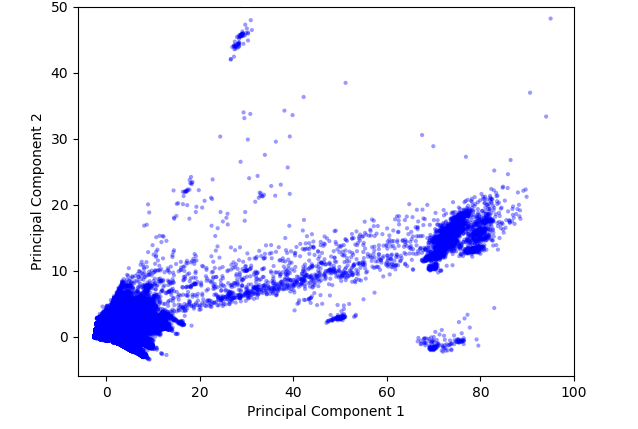
\includegraphics[width=12cm, height=8cm]{./images/single_core_pca}
\centering
\caption{PCA for single core at granularity of 1000}
\label{fig:flow}
\end{figure}

\begin{figure}[h!]
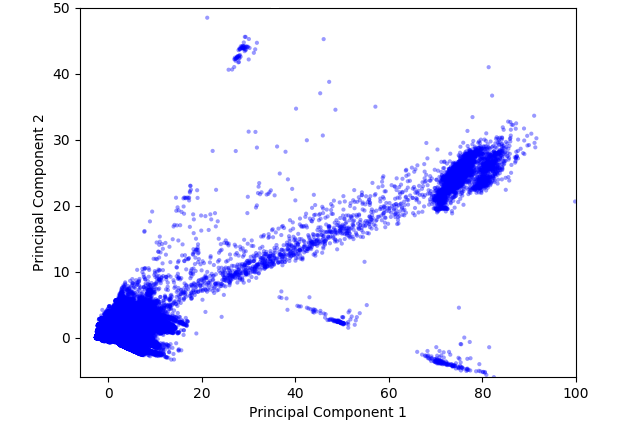
\includegraphics[width=12cm, height=8cm]{./images/dual_no_pca}
\centering
\caption{PCA for dual core with no load at granularity of 1000}
\label{fig:flow}
\end{figure}

\begin{figure}[h!]
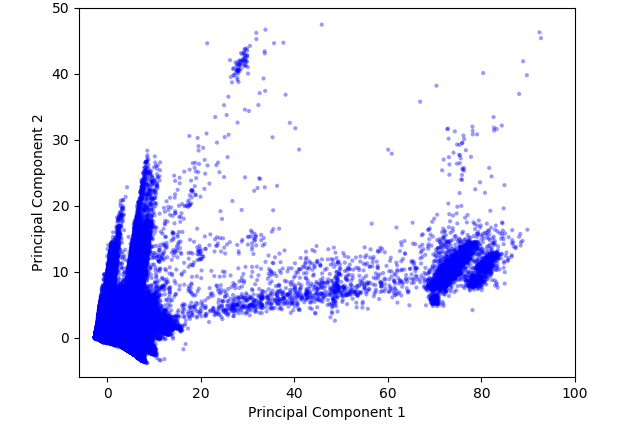
\includegraphics[width=12cm, height=10cm]{./images/dual_full_pca}
\centering
\caption{PCA for dual core with full load at granularity of 1000}
\label{fig:flow}
\end{figure}


\subsection{Correlation Coefficient}
Correlation is widely used statistical concept. Term correlation indicate to mutual relationship between variables or quantities. It is first step to understand the relationship in variables of data. Correlation can indicate or provide information about relationship between variable whether it is casual or intense with other variables. Correlation coefficient provides numerical measure of statistical relationship between two variables. 

\par There are different mathematical techniques are available to calculate correlation coefficient. Such as Pearson technique, Spearman technique, Kendall's Tau technique and many more. In this thesis work we are using Pearson technique. In this thesis work we going to use Pearson technique. We used sklearn[] library from python to calculate correlation coefficient and plot the correlation between each variable. 

\par Values of correlation coefficient for Pearson technique lies between -1 to +1. +1 indicate strongest positive linear relationship whereas -1 indicates the strongest negative linear relationship. We calculated correlation for each hardware performance counter with respect to total cycles to understand the relationship of each of them with total cycles. We calculated correlation coefficient for single core, dual core with no load and dual core with full load for 15 different granularities of training data. We also plotted the heatmap to visualize the relationship of each each hardware counter with other hardware counters i.e. 14x14 correlations. 

\par Following diagrams are correlation coefficient of  training data from single core, dual core with no load and dual core with full load.

\begin{figure}[h!]
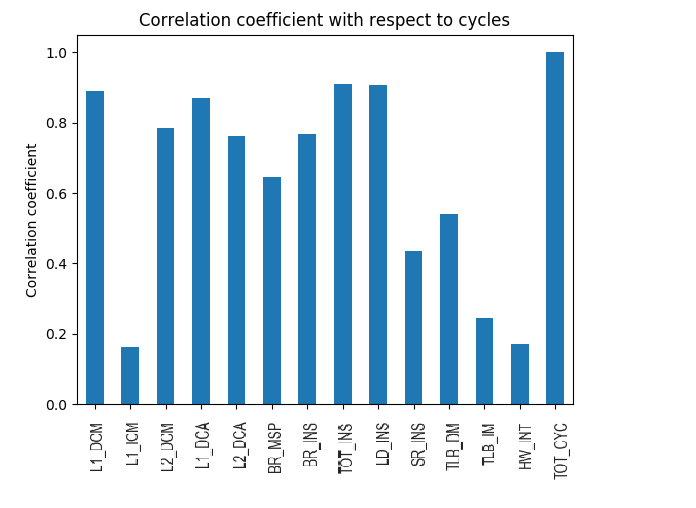
\includegraphics[width=12cm, height=8cm]{./images/CC_single}
\centering
\caption{Correlation coefficient with respect to total cycles on single core}
\label{fig:flow}
\end{figure}

\begin{figure}[h!]
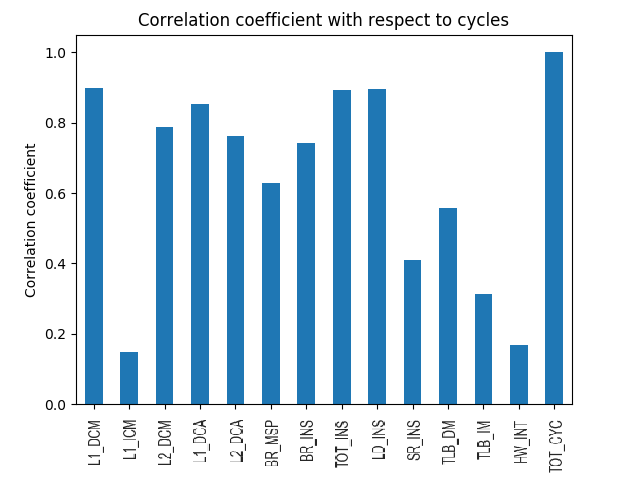
\includegraphics[width=12cm, height=8cm]{./images/CC_no_load}
\centering
\caption{Correlation coefficient with respect to total cycles on dual  core with no load}
\label{fig:flow}
\end{figure}

\begin{figure}[h!]
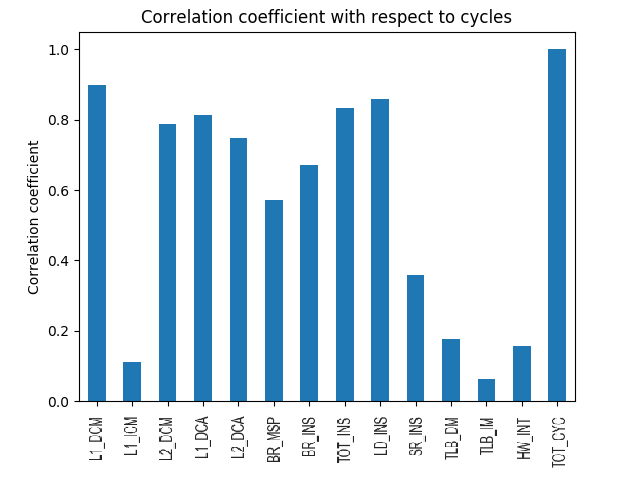
\includegraphics[width=12cm, height=8cm]{./images/CC_full_load}
\centering
\caption{Correlation coefficient with respect to total cycles on dual  core with full load}
\label{fig:flow}
\end{figure}

\begin{figure}[h!]
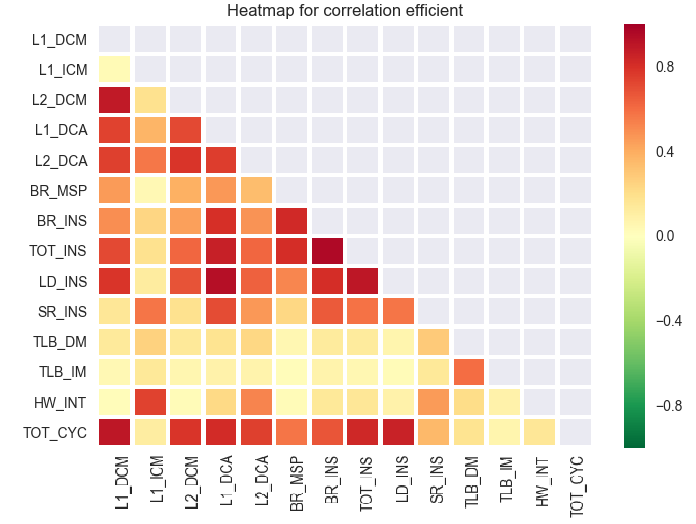
\includegraphics[width=12cm, height=8cm]{./images/heatmap_full_load}
\centering
\caption{Correlation coefficient heatmap for all hardware counters with respect to each other on dual core with full load scenario}
\label{fig:flow}
\end{figure}

\subsection{Hyposthesis of data analysis}
In above section, we saw the two data analysis techniques which are used in this thesis work on training data collected from single core and dual core for both scenarios with 15 different granularities. Visualization of data helps to understand the data and provide more information to draw conclusions for further procedures. 

\par Using PCA, we reduced the data into 2 dimensions and able to relate the data in 2D. Whereas using correlation coefficient, we understood the relationship of each counter with total cycles. Which draws the conclusion that relationship is linear. We can use supervise learning models to predict the performance in terms of cycles. Supervised learning maps input to an output based on input-output pairs. We are going to use 13 dimensional hardware counter data as input and cycles as output. 

\section{Prediction Framework}

 In prediction phase, we are going to use second framework that is prediction framework.  Prediction framework has same structure as training framework to collect the performance data. In addition to training framework, learning model is used to predict the performance of programs. In this framework, training data is used to learn the models. In training data, we have 13 independent variables and single dependent variable. These regression estimates the relationship multiple independent variables and single dependent variable. As our data behavior is linear, we are going to use supervise linear learning techniques like variants of linear regressions. There many learning models are available for linear regression. Following figure \ref{fig:prediction} illustrate the prediction framework. 

\begin{figure}[h!]
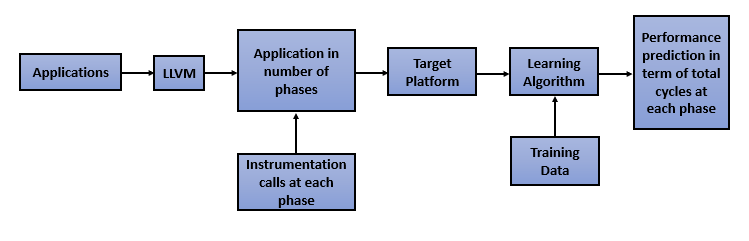
\includegraphics[width=14cm, height=5cm]{./images/prediction}
\centering
\caption{Prediction framework}
\label{fig:prediction}
\end{figure}

After collecting the training data for all hardware counters from 263 training programs, our essential goal is to form a mapping between them in such a way that if new performance data is collected then this mapping can help to estimate the cycles in terms of performance. For given \textit{d}-dimension, $x \in \mathcal{R}^d$ is performance feature vector obtained from host platform and its corresponding timing reference $y \in \mathcal{R}$ is also obtained from hardware platform then mapping function or model ${R}^d$ \textrightarrow ${R}$ is given by , 

\begin{center}
$f(x)=y$
\end{center}

In this section, we are going to discuss the choice of the $f$. We are going to see different variants of linear regression such as Lasso regression, Ridge regression and CLSLR model. 

\subsection{Lasso Regression}
LASSO is acronym for Least Absolute Shrinkage and Selection Operator. The full form of Lasso gives us hint that it is type of linear regression that uses shrinkage. Data values are shrunk toward to mean point. Lasso is simple model with fewer parameters. This model is used for data fitting technique. Objective of lasso is to find the subset predictors that minimizes the prediction error. 

First, lets see the basic linear regression model can be formulated by following equation, where given data set has $n$ points $(x_{i},y_{i})$, for $i = 1,...n$.

$ minimize \theta,   J(\theta) = || X \theta -Y ||^{2 }$ 

Where, $X \in \mathcal{R}^n \times d$ is rows of matrix with $d$ dimensional feature vectors $x_{i}$ and $y \in \mathcal{R}^n$ is column vector $y_{i}$ corresponds to each $x_{i}$. The model $f$ is said to linear when $f(x)=x^{T}\theta$ . such problem is also known as ordinary least square problem.


\par Lasso regression uses L1 regularization. L1 regularizations adds penalty to absolute value of coefficients magnitude. Which can be result in fewer coefficients because some coefficients can become zero and eliminated from the model.  Larger the penalty, closer the value of coefficients to zero which provides simpler model. Goal of the algorithm is to minimize, 

$minimize \theta,  J(\theta)=\dfrac{1}{2n} || X\theta - Y||^{2} + \lambda||\theta||$


Where, $X \in \mathcal{R}^n \times d$ is rows of matrix with $d$ dimensional feature vectors $x_{i}$and $y \in \mathcal{R}^n$ is column vector $y_{i}$ corresponds to each $x_{i}$. The function $f$ remain linear. As we can see in equation is that only difference between ordinary and lasso regression problem is L1 penalty applied to parameter $\theta$. This penalty restrict the $\theta$ to sparse. 

\subsection{Ridge Regression}
Ridge regression is a way to create simple model when number of independent variables are more than predicting or depending variables. Least regression model allows all independent variables regardless whether they are important or not important, which might leads to overfitting of the model and failure to unique solutions. Ridge regression avoid all these problems. 

\par Like lasso regression, ridge regression also uses shrinkage method. Here it uses shrinkage estimator called ridge estimator. Also ridge regression belongs to class of L2 regularization which adds L2 penalty. L2 penalty is equal to square of the magnitude of coefficients. All coefficients are shrunk by same factor so none are eliminated in model. Whereas L1 regularization leads model to be more sparse which is eliminated in ridge regression due to L2 penalty. 

\par Tuning parameter $\lambda$ controls the penalty, if $\lambda = 0$ then ridge regression is similar to least square regression or normal linear regression. When $\lambda = \infty$then all coefficients are shrunk to 0. So ideal value of penalty lies between 0 and $\infty$. Goal of the ridge regression is to minimize $\theta$,

$minimize \theta,  J(\theta)=\dfrac{1}{2n} || X\theta - Y||^{2} + \lambda||\theta||^2$ 

Where, $X \in \mathcal{R}^n \times d$ is rows of matrix with $d$ dimensional feature vectors $x_{i}$and $y \in \mathcal{R}^n$ is column vector $y_{i}$ corresponds to each $x_{i}$. Difference between ridge regression and other regression is that L2 penalty is applied to $\theta$. $\lambda$ is tuning para meter which can change the L2 penalty for model. 

\subsection{Constrained Locally Sparse Linear Regression (CLSLR)}
Assuming the relationship between variables is linear, lasso and ridge regression are expected to have good performance. But if the relationship is non linear then performance of model can suffer. To deal with this issue CLSLR can be used. In CLSLR, L1 penalty is introduced for finding the sparse solution of parameter $\theta$.

\par CLSLR uses euclidean distance between to two unit vectors. The distance $d$ can defined by distance between any two input feature points $x_{i}$ and $x_{j}$ as follows, 

$ d = || \frac{x_{i}}{||x_{i}||} - \frac{x_{j}}{||x_{j}||} ||$

CLSLR solves following optimization problem, 

$minimize \theta_{x_{t}},  J(\theta_{x_{t}})=\dfrac{1}{2m} || X_{x_{t}}\theta_{x_{t}} - Y_{x_{t}}||^{2} + \lambda||\theta||$

where each row $x_{i}$ of the matrix $X_{x_{t}}$ and each row of $y_{i}$ of the matrix $Y_{x_{t}}$ corresponds to points $(x_{i},y_{i})$ in neighborhood $N_{x_{t}}$ with respect to input vector $x_{t}$. CLSLR identifies the $m$-nearest neighbor of $x_{t}$ and solve optimization problem using above equation and obtain $x_{t}$ and compute the prediction by, 

$y_{t} = x_{t}^{T}\theta_{x_{t}}$

\par In prediction phase, performance data is collected and given as input to these algorithm to predict the cycles. These learning algorithms use training data to learn the relationship or mapping the relationship between independent and dependent variables to predict the performance for input data. 





